
\graphicspath{{./chap2/images/}}
\chapter{Connection}
  
\textbf{이 장은 서버와의 연결, 그리고 파일 송수신 방법을 다룬다.}

\section{SSH를 이용한 서버 접속}
	서버는 학교에 있으므로 원격으로만 이용할 수 있다. 이를 위하여 SSH(Secure SHell)를 쓴다. Putty와 같은 전용 프로그램을 이용해도 되고, OpenSSH를 설치한 후 명령 프롬프트와 같은 환경에서 SSH 명령어를 이용해도 된다. 이 문서에서는 후자를, Windows 10 기준으로 설명하도록 하겠다.\\
	
	먼저 윈도우에서 시작 > 설정 > 앱 > 앱 및 기능에 들어간다.
	\begin{figure}[h]
	\begin{center}
        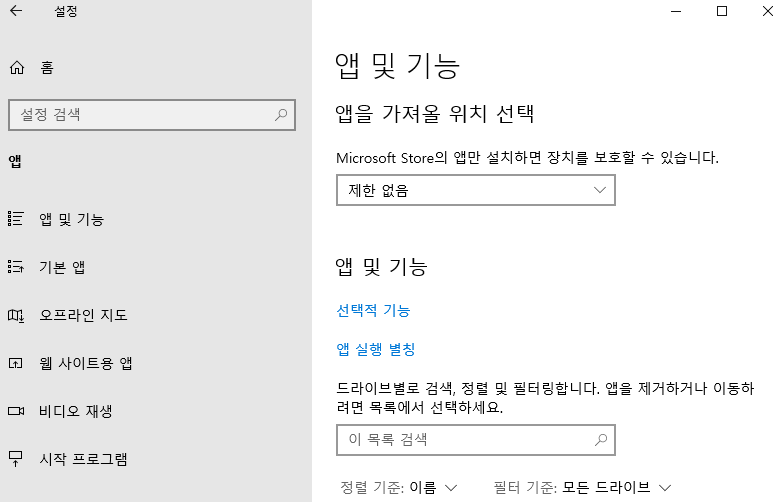
\includegraphics[width=5cm]{ssh1.png}
        \caption{앱 및 기능}
    \end{center}
    \end{figure}
	
	여기서 선택적 기능을 클릭하고 SSH를 검색해 OpenSSH를 찾아 설치한다.
	
	\begin{figure}[H]
	\begin{center}
        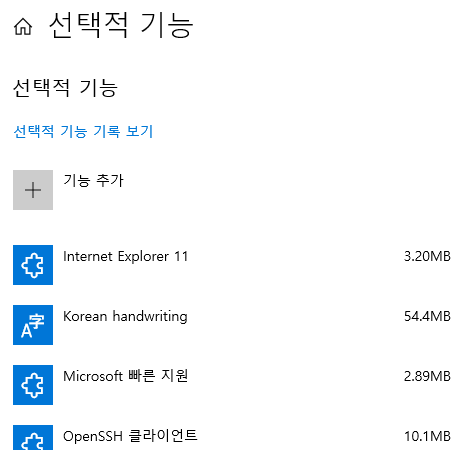
\includegraphics[width=4cm]{ssh2.png}
        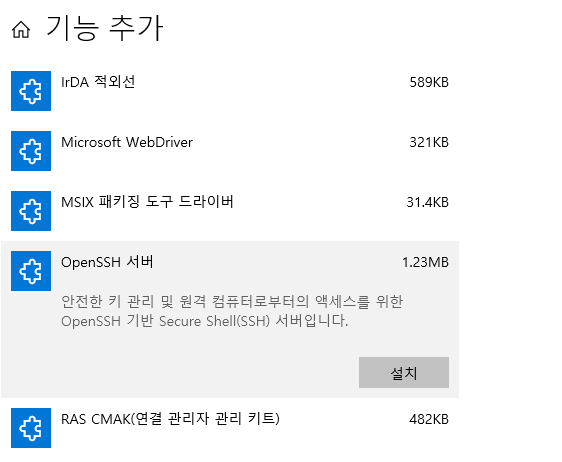
\includegraphics[width=4cm]{ssh3.png}
        \caption{OpenSSH 서버 설치}
    \end{center}
    \end{figure}
    
    이후 관리자 권한으로 cmd나 powershell을 실행한 후 아래 명령어를 입력하면 서버에 접속할 수 있다.
    \begin{lstlisting}
    $ Start-Service sshd
    \end{lstlisting}
    \begin{figure}[H]
	\begin{center}
        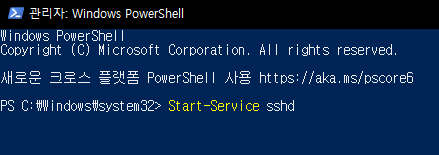
\includegraphics[width=6cm]{ssh4.png}
        \caption{OpenSSH 시작}
    \end{center}
    \end{figure}

	경기과학고등학교 연구용 서버는 Ubuntu 18.04로 구성되어 있다. 이 운영체제는 Windows처럼 사용자 이름(username)과 암호(password)가 있어야 한다. 만약 본인이 서버를 이용하고 싶다면 근처의 정보전공 친구에게 사이다를 사주고 계정을 얻어내도록 하자. 일련의 과정을 통해 서버에 접속할 계정명과 암호, 주소와 포트까지 알게 되었다면 다음과 같은 명령어를 통해 서버에 접속할 수 있다. 이후 암호를 입력하면 접속에 성공한 것이다. 참고로 root 계정은 보통 이용하지 않는다.\\
	\begin{lstlisting}
    $ ssh -p [port] [username]@[address]
      ex) ssh -p 22 root@127.0.0.1
    \end{lstlisting}
    
    
   로그인하면 다음과 같은 화면을 볼 수 있다. 참고로 서버는 TUI 환경이기에 접속된 창으로 모든 작업을 수행하게 된다.
    \begin{figure}[H]
	\begin{center}
        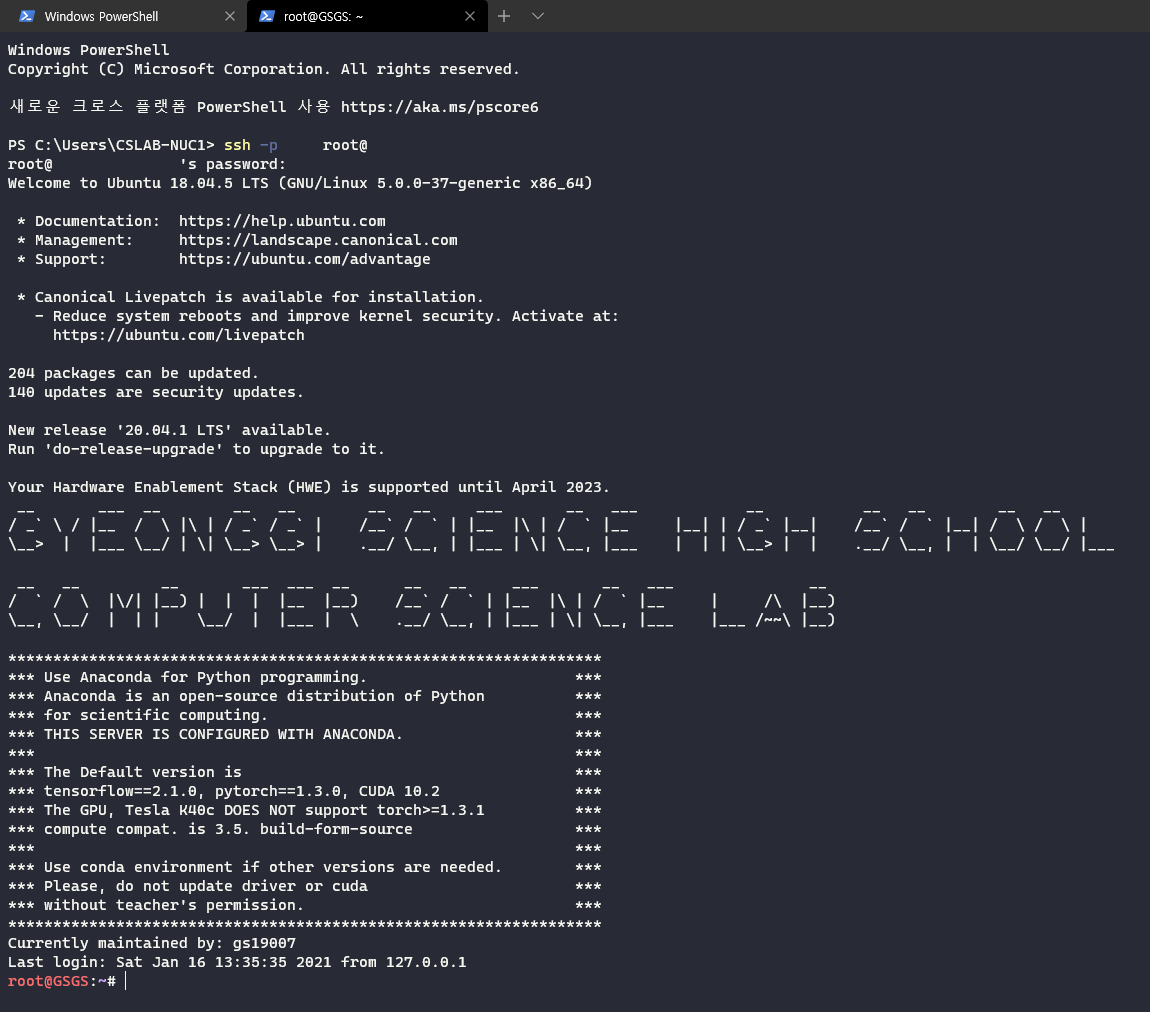
\includegraphics[width=7cm]{ssh5.png}
        \caption{SSH 접속창}
    \end{center}
    \end{figure}
	
\section{SFTP를 이용한 파일 관리}
	SFTP는 SSH File Transfer Protocol의 약어다. 즉, 이미 다룬 SSH 통신을 이용해 파일을 전송하는 것이다. 대표적인 프로그램으로 \href{https://filezilla-project.org/}{FileZilla}가 있다. 파일질라를 설치한 후 좌측 상단 사이트 관리자에서 새 로그인 정보를 만들어 저장하고 연결하면 된다.
	\begin{figure}[H]
	\begin{center}
        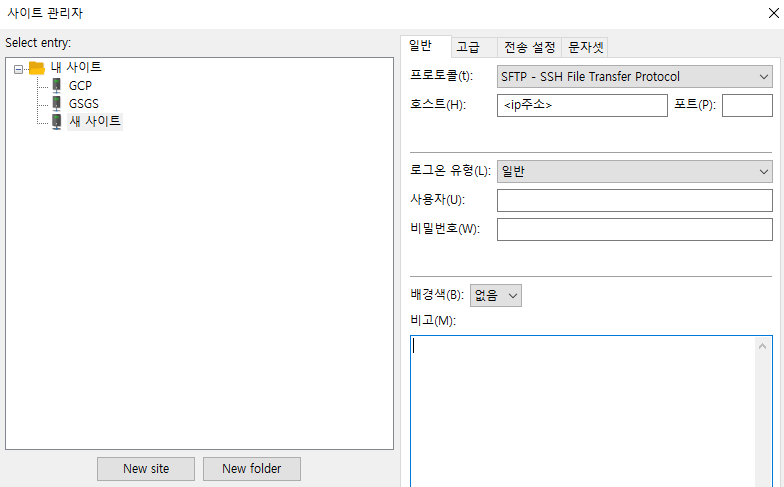
\includegraphics[width=8cm]{sftp2.png}
        \caption{FileZilla 접속}
    \end{center}
    \end{figure}
    접속에 성공하면 화면 양쪽에 파일 탐색기가 생길 것이다. 좌측은 현재 사용자의 컴퓨터이며 우측은 서버다. 이제 사용자는 평소 윈도우 파일 탐색기를 이용하듯 파일을 끌어 옮기거나 다운로드하여 편집할 수 있다. 다만 파일을 다운로드 후 편집하고 다시 업로드를 해야 서버의 파일이 수정된다는 점에 유의해야 한다.
	\begin{figure}[H]
	\begin{center}
        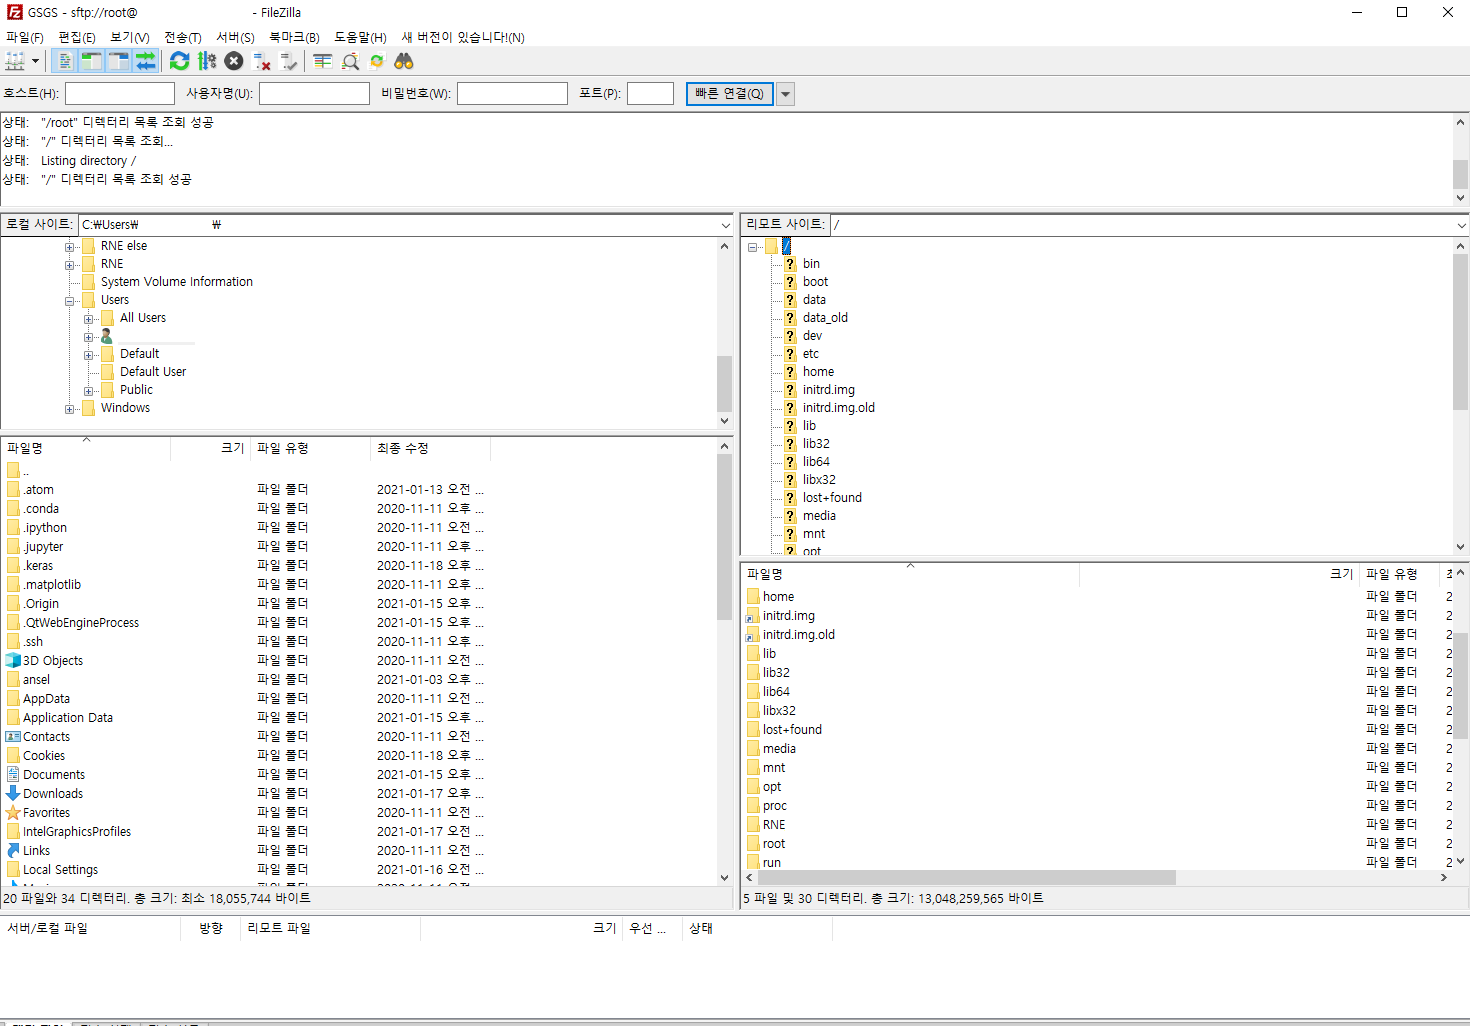
\includegraphics[width=8cm]{sftp3.png}
        \caption{파일질라 접속}
    \end{center}
    \end{figure}
	